\subsubsection{Overview}
The executor constitutes a high-performance zkRollup execution engine implemented in Rust, designed to process Ethereum-compatible transaction batches as the computational backbone of a Layer-2 scaling solution. The architectural philosophy centers on separation of concerns and modular composability. 

\begin{figure}[H]
    \centering
    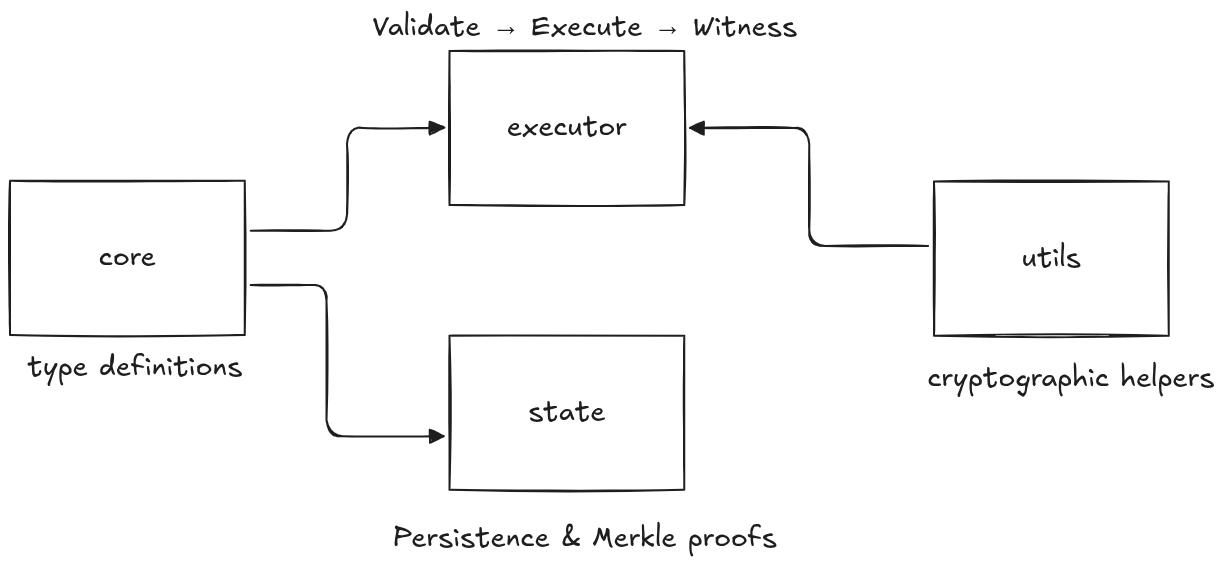
\includegraphics[width=0.75\linewidth]{figures/executor-component-dependency.png}
    \caption{Executor component dependency graph}
    \label{fig:dependency}
\end{figure}

Each module encapsulates a distinct responsibility boundary: core defines the domain vocabulary, executor implements state transition logic, state manages persistent storage with cryptographic commitments, and utils provides cross-cutting cryptographic primitives. This modularization enables independent optimization, testing, and potential substitution of components without cascading changes throughout the system.

\subsubsection{Architectural Components}
The executor architecture comprises four primary modules, each implementing specific design patterns to ensure extensibility and testability.

\subsubsubsection{Core Module (\texttt{src/core/})}

The core module serves as the foundational layer, defining shared types and behavioral contracts used throughout the system. It establishes the domain vocabulary and cryptographic primitives.

\paragraph{File Structure}
The module is organized into the following components:
\begin{itemize}[leftmargin=*, noitemsep]
    \item \texttt{types.rs}: Defines core data structures including \texttt{Account}, \texttt{Transaction}, \texttt{Receipt}, \texttt{Block}, and \texttt{Batch}.
    \item \texttt{command.rs}: Contains the \texttt{TransactionExecutor} trait.
    \item \texttt{rlp.rs}: Handles Ethereum-compatible RLP (Recursive Length Prefix) encoding.
    \item \texttt{batch.rs}: Utilities for processing transaction batches.
\end{itemize}

\paragraph{Key Abstractions}
The architecture relies on several primary types and a specific command pattern to handle state transitions.

\begin{description}[style=nextline, leftmargin=*]
    \item[Key Types] 
    Key data structures include:
    \begin{itemize}
        \item \texttt{Transaction}: Enum variants for \texttt{Transfer}, \texttt{ContractCall}, and \texttt{ContractCreate}. It utilizes \texttt{alloy-primitives} (\texttt{Address}, \texttt{U256}, \texttt{B256}) for Ethereum-native compatibility.
        \item \texttt{Account}: Manages balance, nonce, \texttt{code\_hash}, and \texttt{storage\_root}.
        \item \texttt{Receipt}: Stores execution results and emitted logs.
    \end{itemize}

    \item[The Command Pattern] 
    The \texttt{TransactionCommand} trait (Listing~\ref{lst:command}) encapsulates transaction-specific execution logic, enabling polymorphic handling of transaction variants.
\end{description}

\begin{lstlisting}[style=rustStyle, caption={The Transaction Command Trait}, label={lst:command}]
pub trait TransactionCommand {
    fn execute(&self, state: &mut StateManager, ...) -> Result<...>;
    fn sender(&self) -> &Address;
    // ... other methods
}
\end{lstlisting}

\paragraph{Implementations}
Concrete implementations of the command pattern include:
\begin{itemize}
    \item \textbf{TransferTx}: Handles native balance transfers between accounts.
    \item \textbf{ContractCallTx}: Executes EVM contract calls via the \texttt{EvmExecutor}.
    \item \textbf{ContractCreateTx}: Manages contract deployment logic via the \texttt{EvmExecutor}.
\end{itemize}

\subsubsubsection{Executor Module (\texttt{src/executor/})}

\begin{figure}[H]
    \centering
    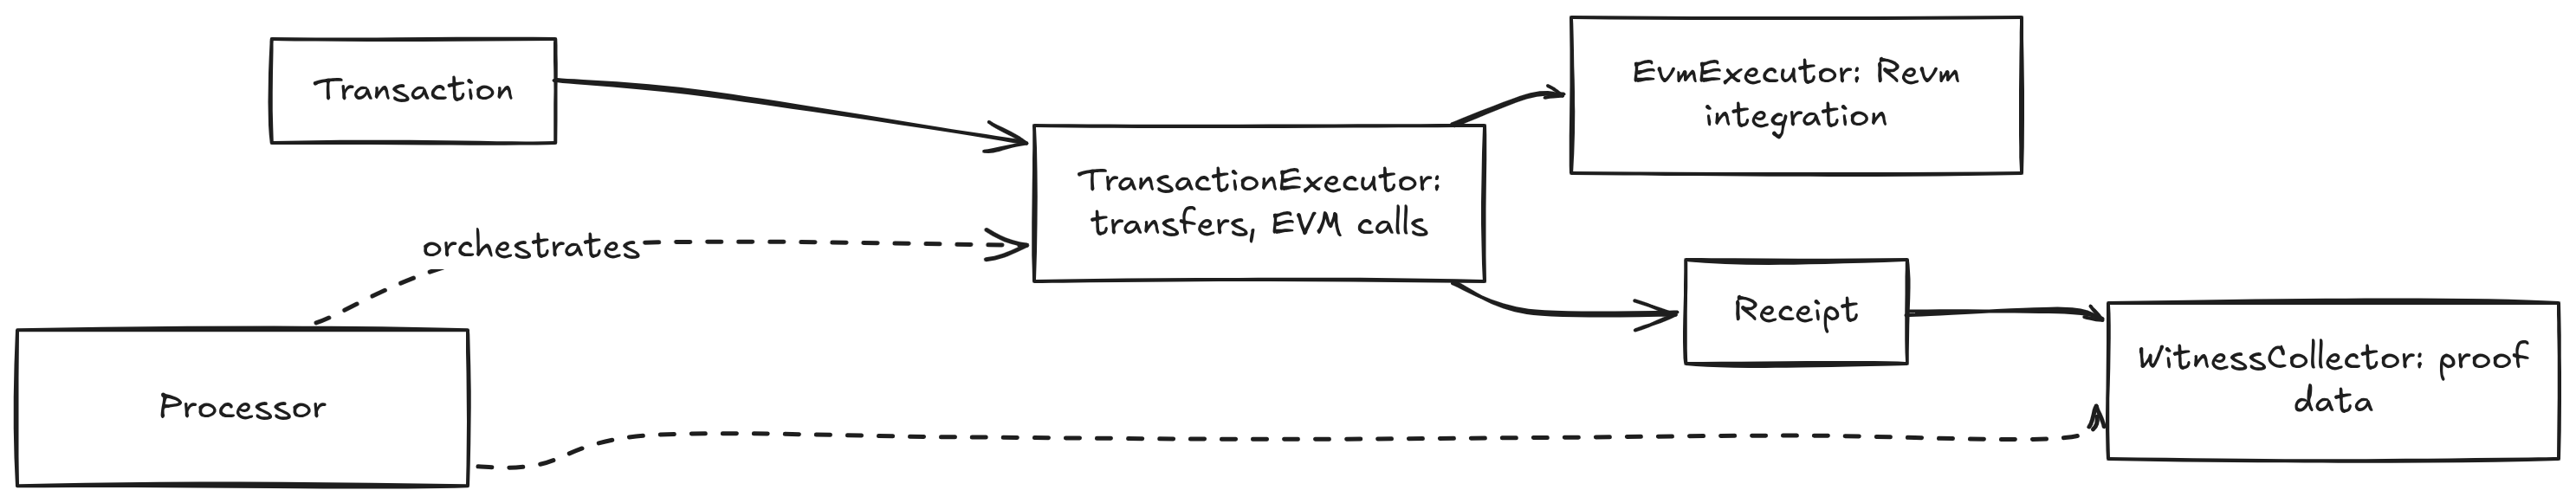
\includegraphics[width=0.75\linewidth]{figures/executor-executor.png}
    \caption{Executor executor module}
    \label{fig:tx_flow}
\end{figure}

The executor module constitutes the primary transaction processing engine. It adheres strictly to the Single Responsibility Principle, separating the concerns of transaction routing and EVM integration.

\paragraph{File Structure}
The module is organized into the following key components:
\begin{itemize}[leftmargin=*, noitemsep]
    \item \texttt{tx\_executor.rs}: Contains the \texttt{TransactionExecutor}, dispatching transactions to transfer logic or the EVM.
    \item \texttt{evm.rs}: Contains the \texttt{EvmExecutor}, which wraps the \textbf{revm} crate for smart contract execution.
    \item \texttt{processor.rs}: The main coordinator that owns the state manager and orchestrates block execution.
\end{itemize}

\paragraph{Key Components and Patterns}
The architecture utilizes several classical design patterns to manage execution complexity and abstract external dependencies.

\begin{description}[style=nextline, leftmargin=*]
    \item[Processor (Facade Pattern)] 
    Acts as the main coordinator for the entire execution subsystem. Clients interact with the \texttt{Processor}, which hides internal complexity, handles batch atomicity (all-or-nothing execution), and orchestrates the transaction lifecycle via methods like \texttt{execute\_transaction()} and \texttt{execute\_block()}.

    \item[TransactionExecutor (Strategy Pattern)] 
    Serves as the transaction dispatcher. It selects the appropriate execution strategy—either native balance transfers or EVM execution—based on the underlying transaction type.

    \item[EvmExecutor (Adapter Pattern)] 
    Acts as the dedicated execution engine. It bridges the internal \texttt{StateRepository} and \texttt{Transaction} types to the interfaces required by the \texttt{revm} crate (\texttt{Database}, \texttt{TxEnv}), safely configuring and running the Ethereum Virtual Machine.
\end{description}

\begin{lstlisting}[style=rustStyle, caption={The Transaction Executor Trait}, label={lst:executor}]
pub trait TransactionExecutor {
    fn execute(&self, state: &mut impl StateRepository) -> Result<Receipt>;
}
\end{lstlisting}

\subsubsubsection{State Module (\texttt{src/state/})}

\begin{figure}[H]
    \centering
    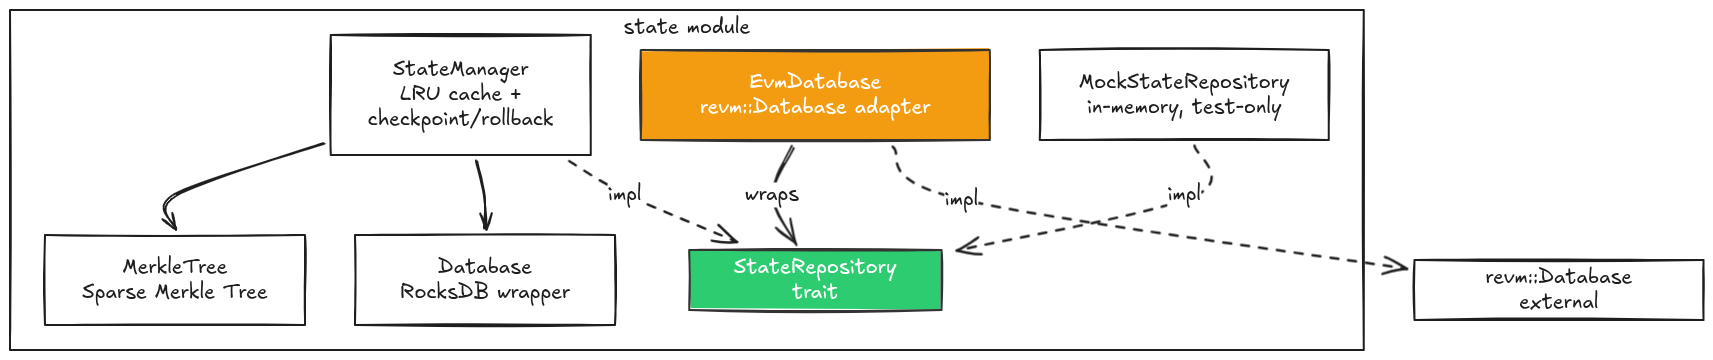
\includegraphics[width=0.75\linewidth]{figures/executor-state.png}
    \caption{Executor state module}
    \label{fig:tx_flow}
\end{figure}

The state module manages data persistence, cryptographic integrity, and efficient state access. It ensures crash consistency and leverages dependency inversion, guaranteeing that high-level execution modules depend on behavioral abstractions rather than concrete storage implementations.

\paragraph{File Structure}
The module is organized into the following components:
\begin{itemize}[leftmargin=*, noitemsep]
    \item \texttt{repository.rs}: Defines the core \texttt{StateRepository} trait.
    \item \texttt{manager.rs}: Contains \texttt{StateManager}, the primary implementation featuring LRU caching, checkpointing, and atomic commits.
    \item \texttt{storage/db.rs}: Provides the \texttt{Database} wrapper around RocksDB for persistent storage.
    \item \texttt{merkle/tree.rs}: Implements a Sparse Merkle Tree (Blake2b) for state root computation.
    \item \texttt{storage/evm\_db.rs}: Contains \texttt{EvmDatabase}, bridging the state manager to the EVM.
    \item \texttt{mock.rs}: Provides \texttt{MockStateRepository}, an in-memory HashMap implementation for testing.
\end{itemize}

\paragraph{Key Components and Patterns}
\begin{description}[style=nextline, leftmargin=*]
    \item[StateRepository (Repository Pattern)] 
    The central abstraction layer. It defines state access operations, allowing the execution logic to remain entirely agnostic to the underlying storage mechanism.

    \item[StateManager] 
    The main state controller implementing the repository trait. It combines Caching (LRU), Atomic Commit, and Snapshot/Restore patterns. It batches database writes to ensure the system never enters a partially updated state.

    \item[EvmDatabase (Adapter Pattern)] 
    Serves as a structural bridge between the internal \texttt{StateRepository} interface and the \texttt{revm::Database} trait.

    \item[MerkleTree] 
    Acts as the system's cryptographic accumulator. It maintains the state tree and generates the State Root, which serves as a verifiable cryptographic commitment to the entire Layer-2 state.
\end{description}

\begin{lstlisting}[style=rustStyle, caption={The State Repository Trait}, label={lst:repository}]
pub trait StateRepository {
    fn get_account(&mut self, addr: &Address) -> Result<Account>;
    fn update_account(&mut self, addr: &Address, account: Account) -> Result<()>;
    fn get_storage(&mut self, addr: &Address, key: &Hash) -> Result<Vec<u8>>;
    fn commit(&mut self) -> Result<Hash>;
    // ... additional storage methods
}
\end{lstlisting}

\subsubsubsection{Utils Module (\texttt{src/utils/})}

The utils module serves as a shared library of cross-cutting concerns, primarily focusing on essential cryptographic primitives and helper functions utilized throughout the entire execution engine. 

\paragraph{File Structure}
\begin{itemize}[leftmargin=*, noitemsep]
    \item \texttt{crypto.rs}: Contains core cryptographic utilities, including hashing and address derivation logic.
\end{itemize}

\paragraph{Key Components}
\begin{description}[style=nextline, leftmargin=*]
    \item[Hashing Operations] 
    Provides standard Ethereum-compatible hashing via \texttt{keccak256}, which is foundational for data integrity checks, state root generation, and transaction hashing.

    \item[Address Derivation] 
    Contains \texttt{public\_key\_to\_address} logic, mapping cryptographic public keys to standard 20-byte Ethereum addresses.
\end{description}

\subsubsection{Operational Flow}

\begin{figure}[H]
    \centering
    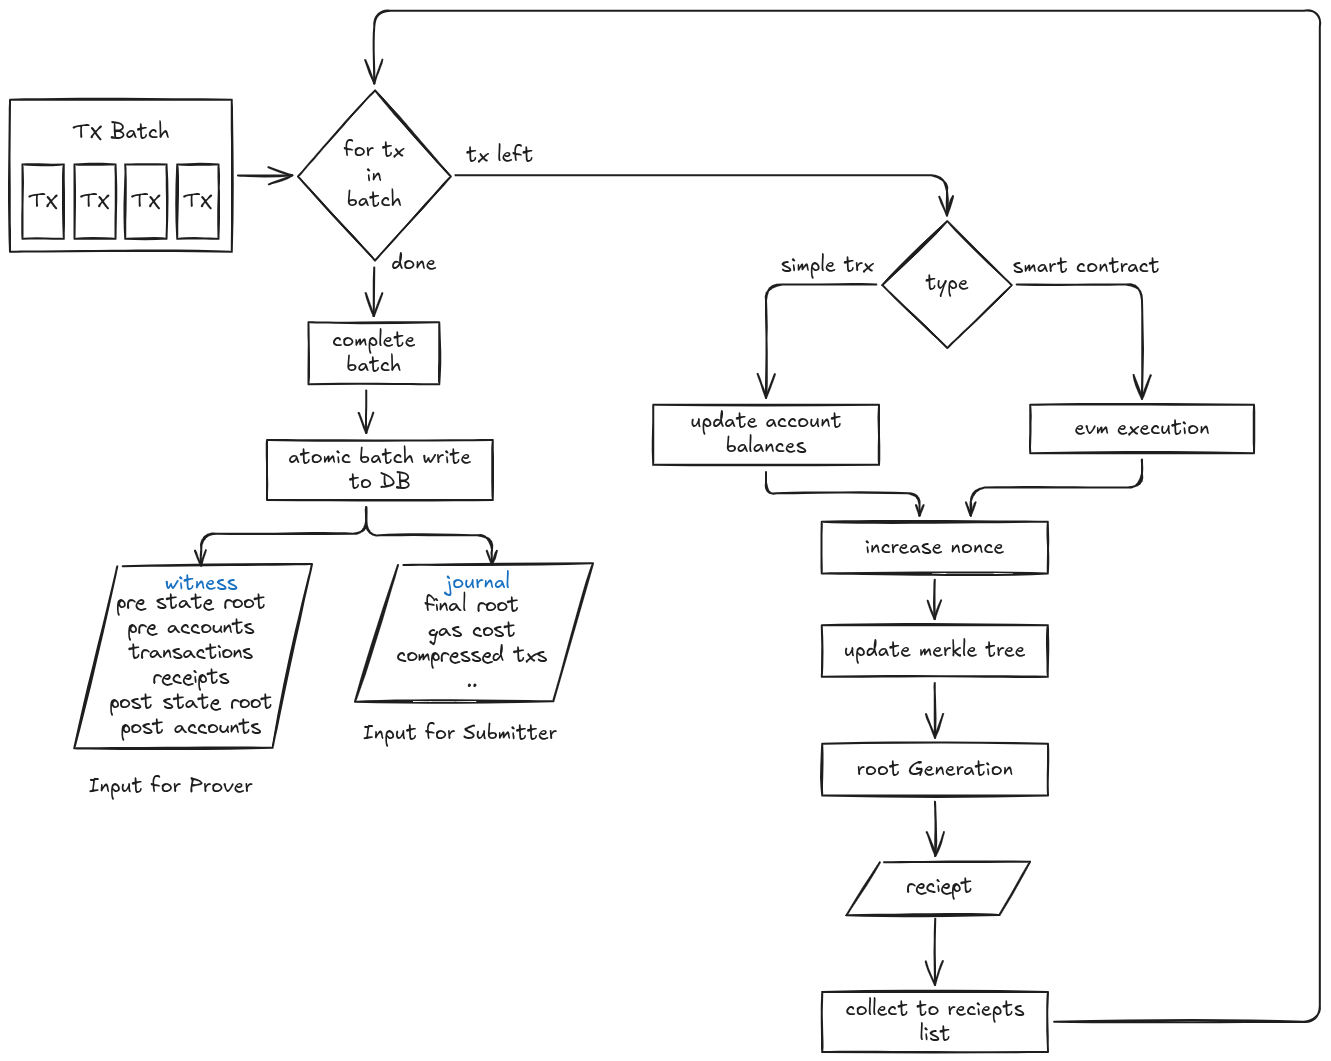
\includegraphics[width=0.75\linewidth]{figures/executor-tx-flow.png}
    \caption{Executor transaction flow}
    \label{fig:tx_flow}
\end{figure}

\begin{figure}[H]
    \centering
    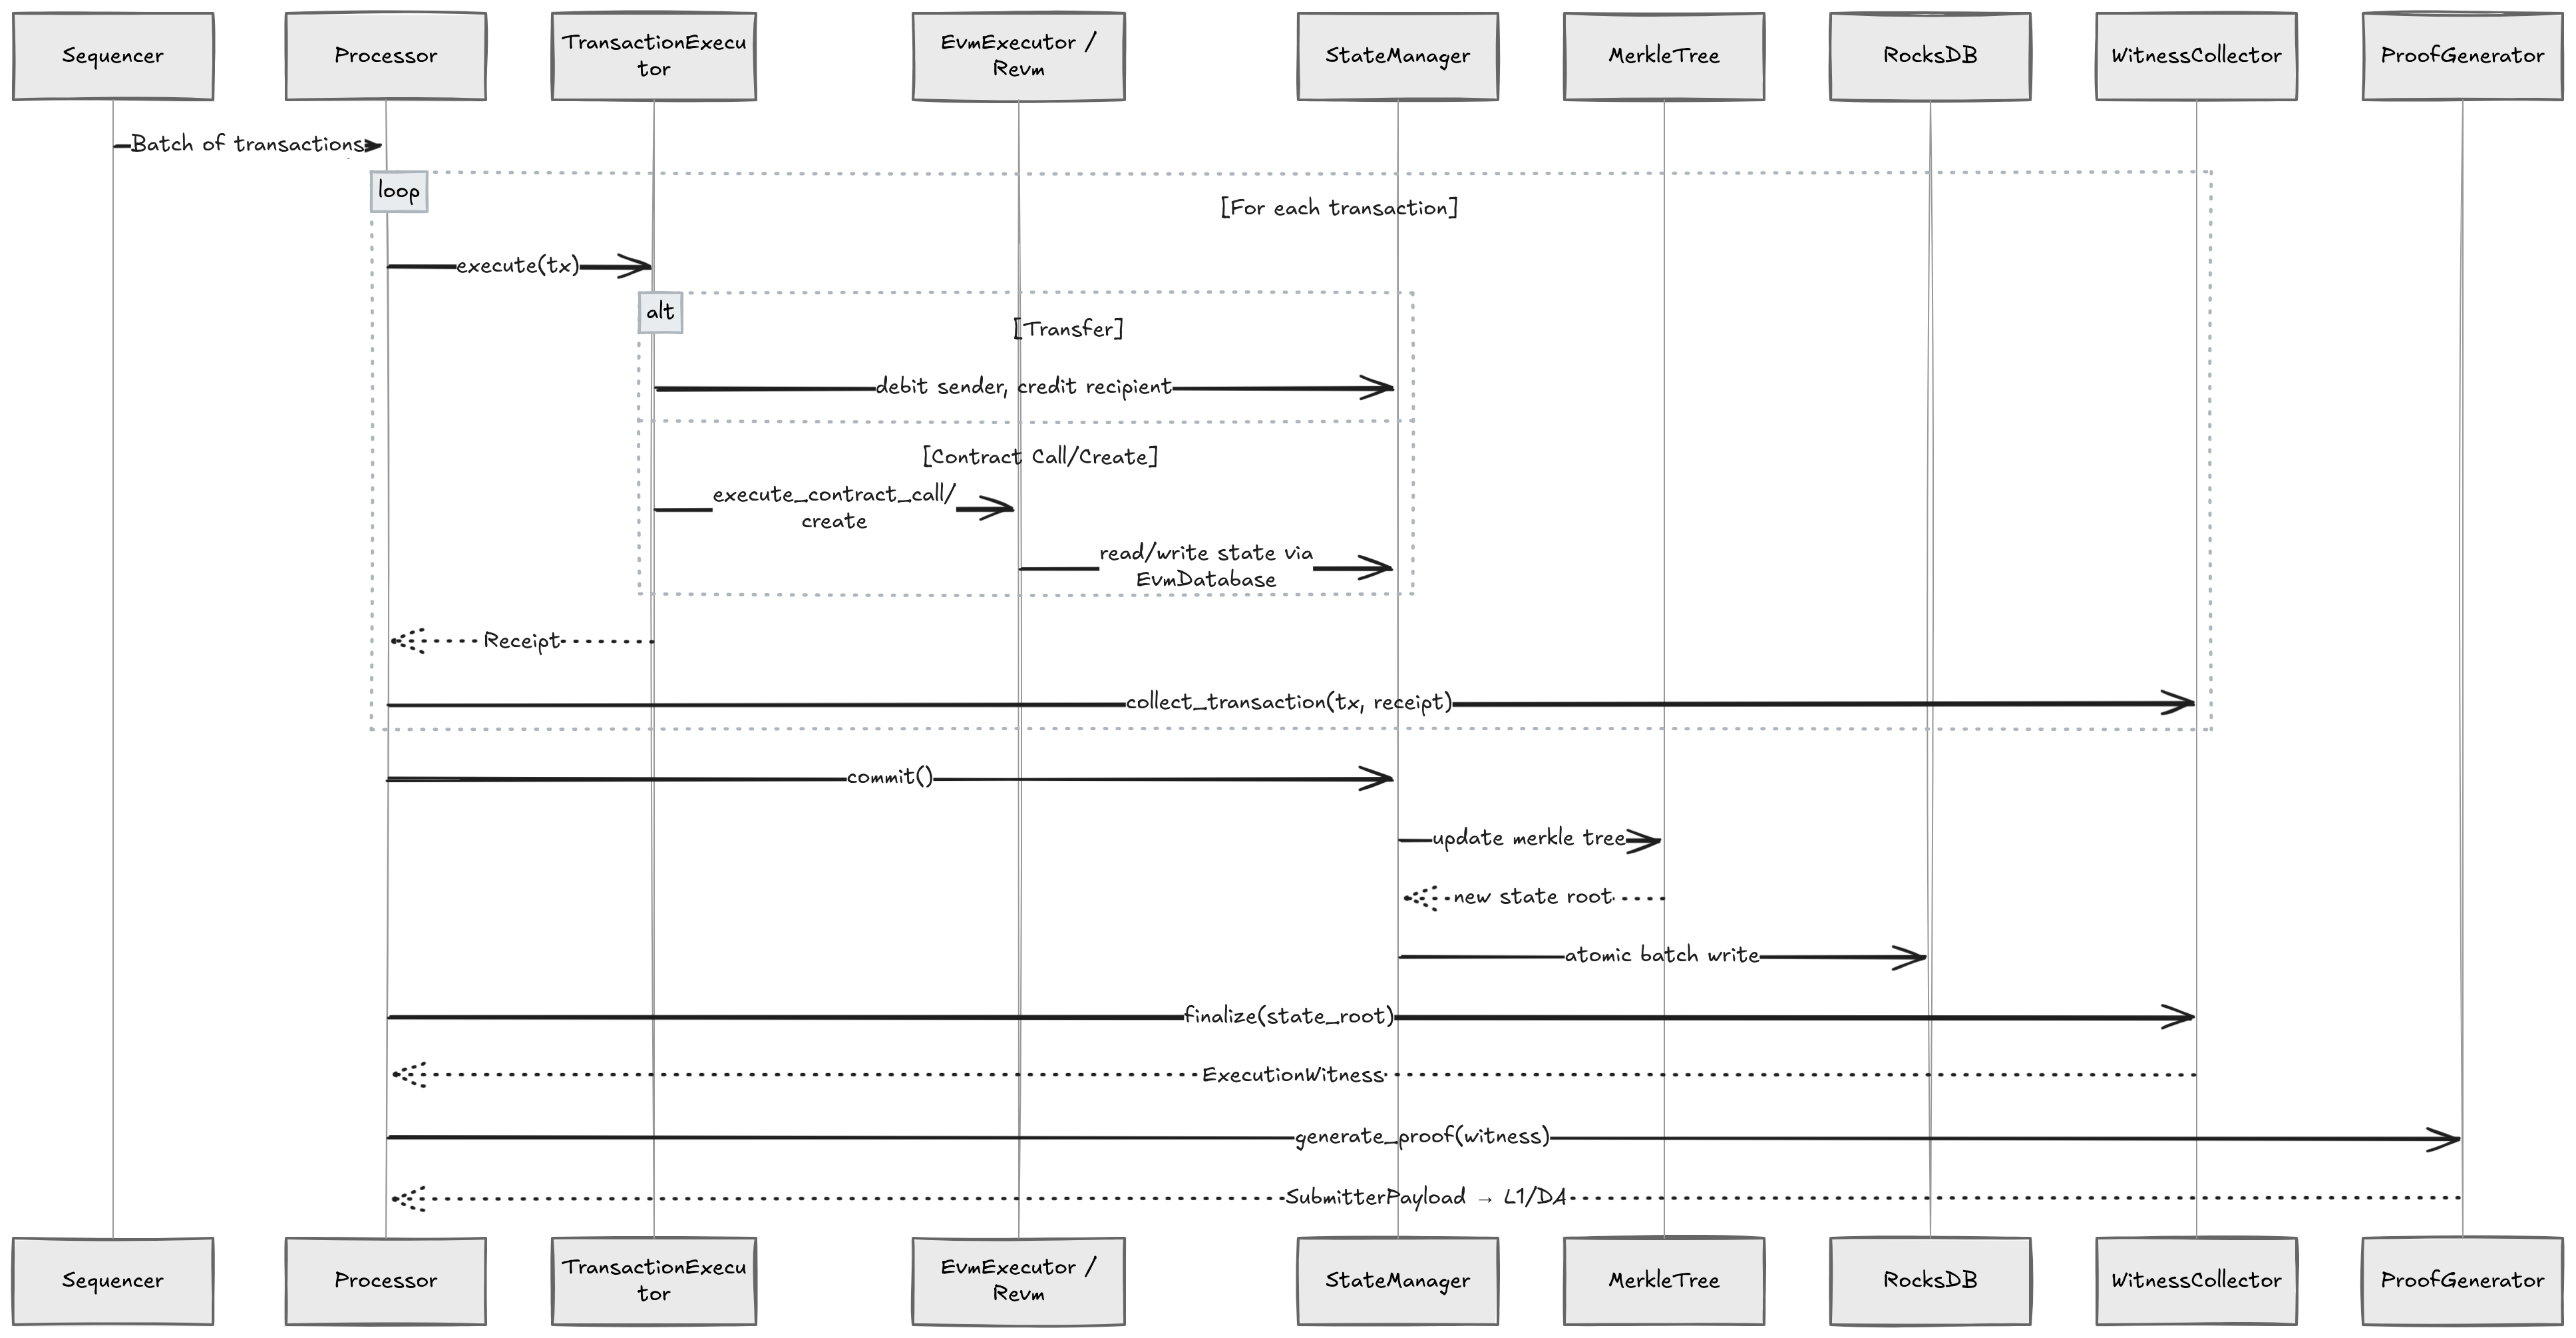
\includegraphics[width=0.75\linewidth]{figures/executor-flow.png}
    \caption{Executor sequence diagram}
    \label{fig:tx_flow}
\end{figure}

\paragraph{Phase 1: Execution (Executor Module)}
Transaction dispatch occurs based on type:
\begin{itemize}[leftmargin=*]
    \item \textbf{Transfer}: Direct state mutation via \texttt{StateRepository} (debit sender, credit recipient).
    \item \textbf{Contract Operations}: Delegation to \texttt{EvmExecutor}, which instantiates \texttt{revm::Evm} with an \texttt{EvmDatabase} adapter bridging to \texttt{StateRepository}.
\end{itemize}

\paragraph{Phase 2: State Commitment (State Module)}
Post-execution, \texttt{StateManager::commit()} performs:
\begin{enumerate}[leftmargin=*]
    \item Collection of dirty accounts from pending write set
    \item Serialization via \texttt{bincode}
    \item Merkle tree updates with new state root computation
    \item Atomic batch write to RocksDB (all-or-nothing persistence)
\end{enumerate}

\subsubsection{Design Rationale and Trade-offs}
\label{sec:rationale}

\paragraph{Modular Separation vs. Performance}
The strict module separation introduces interface overhead but yields critical benefits:
\begin{itemize}[leftmargin=*]
    \item \textbf{Testability}: Mock implementations enable unit testing without database instantiation ($<$1ms vs. disk I/O).
    \item \textbf{Swappability}: Storage engines (RocksDB $\rightarrow$ LMDB) are interchangeable without cascading changes.
    \item \textbf{Parallel Development}: Team members can own modules with minimal merge conflicts.
\end{itemize}

\paragraph{Alloy Primitives Adoption}
Standardizing on \texttt{alloy-primitives} (\texttt{Address}, \texttt{U256}, \texttt{B256}) rather than custom types:
\begin{itemize}[leftmargin=*]
    \item[\cmark] Zero-cost interop with \texttt{revm} (shared type system)
    \item[\cmark] Battle-tested 256-bit arithmetic (security critical)
    \item[\cmark] Native RLP encoding via \texttt{alloy-rlp}
    \item[\xmark] Dependency on external crate evolution
\end{itemize}

\paragraph{Revm Integration vs. Custom EVM}
Using \texttt{revm} rather than a custom EVM implementation:
\begin{itemize}[leftmargin=*]
    \item[\cmark] Production-tested (used by Reth, Foundry)
    \item[\cmark] Complete opcode and precompile support
    \item[\cmark] Trait-based \texttt{Database} interface enables state layer decoupling
    \item[\xmark] Binary size overhead
\end{itemize}

\paragraph{Sparse Merkle Tree Selection}
Blake2b-based SMT chosen over alternatives:
\begin{itemize}[leftmargin=*]
    \item[\cmark] Efficient for sparse key spaces (typical blockchain state)
    \item[\cmark] Faster than SHA-256 in most environments
    \item[\xmark] Less standard than SHA-256 for external verification
\end{itemize}

\paragraph{LRU Cache Sizing}
10K account / 50K storage slot cache limits represent a balance between:
\begin{itemize}[leftmargin=*]
    \item Hit rate optimization (typical block access patterns show locality)
    \item Memory constraints (bounded usage prevents OOM in long-running nodes)
    \item Checkpoint overhead (larger caches increase rollback memory)
\end{itemize}

\paragraph{Nonce Increment Timing}
Nonces increment \textit{after} execution:
\begin{itemize}[leftmargin=*]
    \item Matches Ethereum semantics where reverted transactions still consume nonces
    \item Requires careful handling of out-of-gas scenarios in EVM execution
\end{itemize}



\subsubsection{Integration with Other Components}
\label{sec:integration}

The executor crate interfaces with key external system categories, acting as the central state-transition engine within the broader Layer-2 architecture:

\paragraph{Sequencer Integration}
The sequencer submits transaction batches via the \texttt{Batch} struct:
\begin{itemize}[leftmargin=*]
    \item \textbf{Interface}: Binary serialization (\texttt{bincode}) over network transport.
    \item \textbf{Contract}: The sequencer guarantees transaction ordering and data availability; the executor guarantees deterministic execution and state transitions.
    \item \textbf{Backpressure}: Executor TPS vs. Sequencer ingestion rate is managed dynamically via block batch sizing.
\end{itemize}

\paragraph{Zero-Knowledge Prover Integration}
The executor acts as the host/witness generator for an external prover system (e.g., a decentralized prover network or dedicated zkVM hardware):
\begin{itemize}[leftmargin=*]
    \item \textbf{Data Handoff}: The executor constructs an \texttt{ExecutionWitness} containing pre/post state roots, transaction receipts, and all necessary Merkle inclusion proofs.
    \item \textbf{Adapter Pattern}: Specific prover SDKs (such as RISC Zero or SP1) are isolated behind generic adapter traits, preventing vendor lock-in and allowing seamless prover substitution.
    \item \textbf{Stateless Proving}: Because the witness contains all required cryptographic data, the external prover can deterministically verify the state transition without needing access to the executor's RocksDB database.
\end{itemize}

\paragraph{Data Availability Layer \& Layer-1}
Post-execution and proving, the system outputs data for on-chain storage and verification:
\begin{itemize}[leftmargin=*]
    \item \textbf{Journal}: Public inputs intended for the Layer-1 verifier contract (post-state root, block number, gas used) to update the rollup's canonical state.
    \item \textbf{Batch Data}: Compressed transaction data submitted to the Data Availability (DA) layer to ensure state reconstruction is always possible.
\end{itemize}

\begin{table}[H]
\centering
\caption{External Dependencies and Integration Points}
\label{tab:dependencies}
\begin{tabular}{@{}llll@{}}
\toprule
\textbf{Category} & \textbf{Crate} & \textbf{Version} & \textbf{Purpose} \\
\midrule
Ethereum Types & \texttt{alloy-primitives} & 0.6+ & Address, U256, B256 \\
RLP Encoding & \texttt{alloy-rlp} & 0.6+ & Transaction hashing \\
EVM Execution & \texttt{revm} & 8.0+ & Smart contract runtime \\
Cryptography & \texttt{tiny-keccak} & 2.0+ & Hashing \\
Storage & \texttt{rocksdb} & 0.21+ & Persistent KV store \\
Merkle Trees & \texttt{sparse-merkle-tree} & 0.6+ & State commitments \\
Serialization & \texttt{serde}, \texttt{bincode} & 1.0+, 1.3+ & Wire format \\
\bottomrule
\end{tabular}
\end{table}

The dependency stack prioritizes \textbf{pure Rust} implementations where possible to eliminate C FFI complications during cross-compilation, a critical requirement for generating compatible execution witnesses for RISC-V-based zkVM environments.